\documentclass[tikz,border=2pt]{standalone}
\usepackage{amsmath}
\usepackage{pgfplots}
\pgfplotsset{compat=1.18}

\begin{document}
% An increasing sequence never steps down (a_{n+1} >= a_n); a decreasing one never steps up.
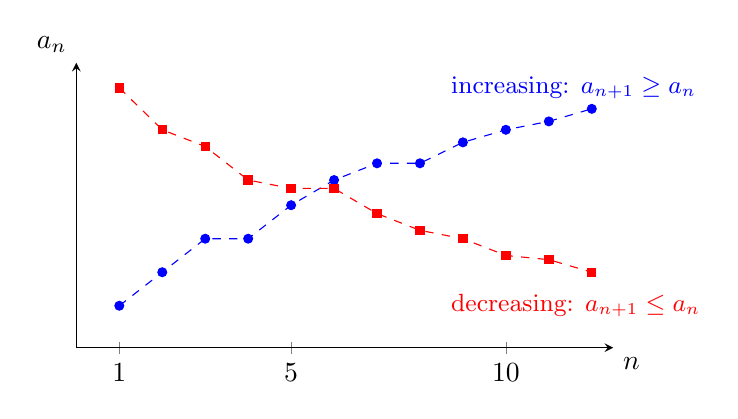
\begin{tikzpicture}
	\begin{axis}[
		axis lines=middle,
		xmin=0, xmax=12.5,
		ymin=0, ymax=3.4,
		xtick={1,5,10}, ytick=\empty,
		xlabel={$n$}, ylabel={$a_n$},
		xlabel style={below right}, ylabel style={above left},
		clip=false,
		width=8.4cm, height=5.2cm
		]
		\addplot[blue, thin, dashed, mark=*, mark size=1.6pt, mark options={solid}] coordinates {(1,0.5) (2,0.9) (3,1.3) (4,1.3) (5,1.7) (6,2.0) (7,2.2) (8,2.2) (9,2.45) (10,2.6) (11,2.7) (12,2.85)};
		\addplot[red, thin, dashed, mark=square*, mark size=1.5pt, mark options={solid}] coordinates {(1,3.1) (2,2.6) (3,2.4) (4,2.0) (5,1.9) (6,1.9) (7,1.6) (8,1.4) (9,1.3) (10,1.1) (11,1.05) (12,0.9)};
		\node[blue, anchor=west, font=\small] at (axis cs:8.5,3.1) {increasing: $a_{n+1}\ge a_n$};
		\node[red, anchor=west, font=\small] at (axis cs:8.5,0.5) {decreasing: $a_{n+1}\le a_n$};
	\end{axis}
\end{tikzpicture}
\end{document}
